\FloatBarrier
\begin{figure}[!h]
\centering
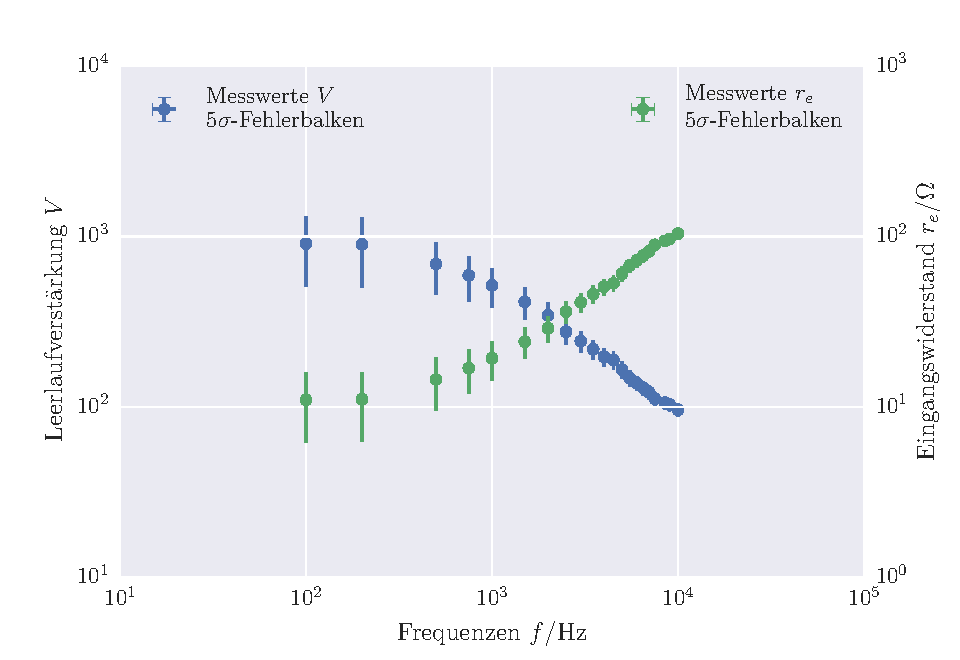
\includegraphics[scale=1]{../Grafiken/Amperemeter_Leerlaufverstaerkung_Eingangswiderstand.pdf}
\caption{Doppellogarithmische Darstellung des Leerlaufverstärkung (linke Skala) und des Eingangswiderstandes 
	(rechte Skala) der Amperemeterschaltung in Abhängigkeit der
	Frequenz.\label{fig:amperemeter_leerlaufverstaerkung_eingangswiderstand}}
\end{figure}
\FloatBarrier